% generated by gen_phase_fig.py -- do not edit by hand
\documentclass[10pt]{standalone}
\usepackage{mathptmx}
\usepackage{tikz}
\usetikzlibrary{arrows.meta}
\definecolor{cval}{HTML}{7030A0}
\definecolor{cload}{HTML}{EEE8AA}
\definecolor{cstore}{HTML}{FAD7B5}
\definecolor{cfpu}{HTML}{B4E7EA}
\definecolor{cwake}{HTML}{DDDDDD}
\newcommand{\fs}{\fontsize{6.6}{7.6}\selectfont}
\newcommand{\fss}{\fontsize{5.7}{6.6}\selectfont}
\begin{document}
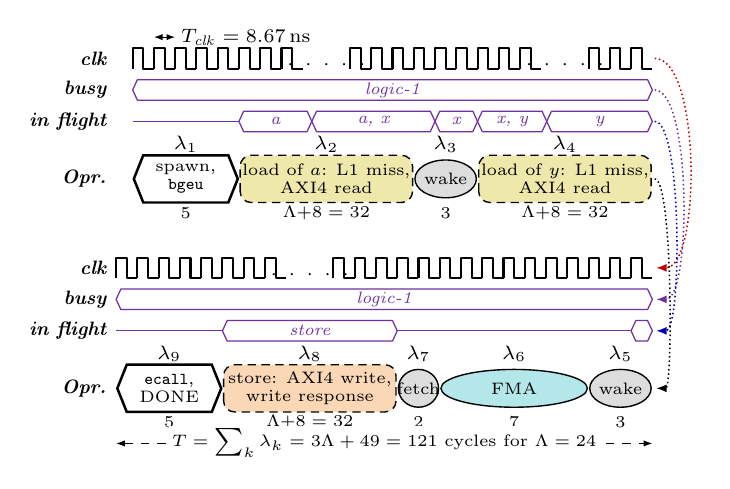
\begin{tikzpicture}[x=1cm, y=1cm,
  sig/.style={font=\fs\bfseries\itshape, anchor=east, inner sep=0.5pt},
  val/.style={font=\fss\itshape, text=cval, inner sep=0.5pt},
  wire/.style={line width=0.75pt, line join=round},
  thin/.style={line width=0.45pt, line join=round, draw=cval},
  lam/.style={font=\fs, inner sep=0.5pt},
  lab/.style={font=\fss, align=center, inner sep=0.5pt},
  dim/.style={{Latex[length=1.1mm, width=0.8mm]}-{Latex[length=1.1mm, width=0.8mm]}, line width=0.4pt, dashed},
  conn/.style={-{Latex[length=1.3mm, width=1mm]}, line width=0.55pt, densely dotted}]

\node[sig] at (1.020,-0.390) {clk};
\node[sig] at (1.020,-0.790) {busy};
\node[sig] at (1.020,-1.190) {in flight};
\node[sig] at (1.020,-1.920) {Opr.};
\node[sig] at (1.020,-3.050) {clk};
\node[sig] at (1.020,-3.450) {busy};
\node[sig] at (1.020,-3.850) {in flight};
\node[sig] at (1.020,-4.580) {Opr.};
\draw[wire] (1.330,-0.520) -- (1.330,-0.260) -- (1.465,-0.260) -- (1.465,-0.520) -- (1.600,-0.520);
\draw[wire] (1.600,-0.520) -- (1.600,-0.260) -- (1.735,-0.260) -- (1.735,-0.520) -- (1.870,-0.520);
\draw[wire] (1.870,-0.520) -- (1.870,-0.260) -- (2.005,-0.260) -- (2.005,-0.520) -- (2.140,-0.520);
\draw[wire] (2.140,-0.520) -- (2.140,-0.260) -- (2.275,-0.260) -- (2.275,-0.520) -- (2.410,-0.520);
\draw[wire] (2.410,-0.520) -- (2.410,-0.260) -- (2.545,-0.260) -- (2.545,-0.520) -- (2.680,-0.520);
\draw[wire] (2.680,-0.520) -- (2.680,-0.260) -- (2.815,-0.260) -- (2.815,-0.520) -- (2.950,-0.520);
\draw[wire] (2.950,-0.520) -- (2.950,-0.260) -- (3.085,-0.260) -- (3.085,-0.520) -- (3.220,-0.520);
\draw[wire] (3.220,-0.520) -- (3.220,-0.260) -- (3.355,-0.260) -- (3.355,-0.520) -- (3.490,-0.520);
\draw[wire] (4.090,-0.520) -- (4.090,-0.260) -- (4.225,-0.260) -- (4.225,-0.520) -- (4.360,-0.520);
\draw[wire] (4.360,-0.520) -- (4.360,-0.260) -- (4.495,-0.260) -- (4.495,-0.520) -- (4.630,-0.520);
\draw[wire] (4.630,-0.520) -- (4.630,-0.260) -- (4.765,-0.260) -- (4.765,-0.520) -- (4.900,-0.520);
\node[font=\fs] at (3.790,-0.480) {$\cdot\;\cdot\;\cdot\;\cdot\;\cdot$};
\draw[wire] (4.900,-0.520) -- (4.900,-0.260) -- (5.035,-0.260) -- (5.035,-0.520) -- (5.170,-0.520);
\draw[wire] (5.170,-0.520) -- (5.170,-0.260) -- (5.305,-0.260) -- (5.305,-0.520) -- (5.440,-0.520);
\draw[wire] (5.440,-0.520) -- (5.440,-0.260) -- (5.575,-0.260) -- (5.575,-0.520) -- (5.710,-0.520);
\draw[wire] (5.710,-0.520) -- (5.710,-0.260) -- (5.845,-0.260) -- (5.845,-0.520) -- (5.980,-0.520);
\draw[wire] (5.980,-0.520) -- (5.980,-0.260) -- (6.115,-0.260) -- (6.115,-0.520) -- (6.250,-0.520);
\draw[wire] (6.250,-0.520) -- (6.250,-0.260) -- (6.385,-0.260) -- (6.385,-0.520) -- (6.520,-0.520);
\draw[wire] (7.120,-0.520) -- (7.120,-0.260) -- (7.255,-0.260) -- (7.255,-0.520) -- (7.390,-0.520);
\draw[wire] (7.390,-0.520) -- (7.390,-0.260) -- (7.525,-0.260) -- (7.525,-0.520) -- (7.660,-0.520);
\draw[wire] (7.660,-0.520) -- (7.660,-0.260) -- (7.795,-0.260) -- (7.795,-0.520) -- (7.930,-0.520);
\node[font=\fs] at (6.820,-0.480) {$\cdot\;\cdot\;\cdot\;\cdot\;\cdot$};
\draw[wire] (7.660,-3.180) -- (7.660,-2.920) -- (7.795,-2.920) -- (7.795,-3.180) -- (7.930,-3.180);
\draw[wire] (7.390,-3.180) -- (7.390,-2.920) -- (7.525,-2.920) -- (7.525,-3.180) -- (7.660,-3.180);
\draw[wire] (7.120,-3.180) -- (7.120,-2.920) -- (7.255,-2.920) -- (7.255,-3.180) -- (7.390,-3.180);
\draw[wire] (6.850,-3.180) -- (6.850,-2.920) -- (6.985,-2.920) -- (6.985,-3.180) -- (7.120,-3.180);
\draw[wire] (6.580,-3.180) -- (6.580,-2.920) -- (6.715,-2.920) -- (6.715,-3.180) -- (6.850,-3.180);
\draw[wire] (6.310,-3.180) -- (6.310,-2.920) -- (6.445,-2.920) -- (6.445,-3.180) -- (6.580,-3.180);
\draw[wire] (6.040,-3.180) -- (6.040,-2.920) -- (6.175,-2.920) -- (6.175,-3.180) -- (6.310,-3.180);
\draw[wire] (5.770,-3.180) -- (5.770,-2.920) -- (5.905,-2.920) -- (5.905,-3.180) -- (6.040,-3.180);
\draw[wire] (5.500,-3.180) -- (5.500,-2.920) -- (5.635,-2.920) -- (5.635,-3.180) -- (5.770,-3.180);
\draw[wire] (5.230,-3.180) -- (5.230,-2.920) -- (5.365,-2.920) -- (5.365,-3.180) -- (5.500,-3.180);
\draw[wire] (4.960,-3.180) -- (4.960,-2.920) -- (5.095,-2.920) -- (5.095,-3.180) -- (5.230,-3.180);
\draw[wire] (4.690,-3.180) -- (4.690,-2.920) -- (4.825,-2.920) -- (4.825,-3.180) -- (4.960,-3.180);
\draw[wire] (4.420,-3.180) -- (4.420,-2.920) -- (4.555,-2.920) -- (4.555,-3.180) -- (4.690,-3.180);
\draw[wire] (4.150,-3.180) -- (4.150,-2.920) -- (4.285,-2.920) -- (4.285,-3.180) -- (4.420,-3.180);
\draw[wire] (3.880,-3.180) -- (3.880,-2.920) -- (4.015,-2.920) -- (4.015,-3.180) -- (4.150,-3.180);
\draw[wire] (3.010,-3.180) -- (3.010,-2.920) -- (3.145,-2.920) -- (3.145,-3.180) -- (3.280,-3.180);
\draw[wire] (2.740,-3.180) -- (2.740,-2.920) -- (2.875,-2.920) -- (2.875,-3.180) -- (3.010,-3.180);
\draw[wire] (2.470,-3.180) -- (2.470,-2.920) -- (2.605,-2.920) -- (2.605,-3.180) -- (2.740,-3.180);
\node[font=\fs] at (3.580,-3.140) {$\cdot\;\cdot\;\cdot\;\cdot\;\cdot$};
\draw[wire] (2.200,-3.180) -- (2.200,-2.920) -- (2.335,-2.920) -- (2.335,-3.180) -- (2.470,-3.180);
\draw[wire] (1.930,-3.180) -- (1.930,-2.920) -- (2.065,-2.920) -- (2.065,-3.180) -- (2.200,-3.180);
\draw[wire] (1.660,-3.180) -- (1.660,-2.920) -- (1.795,-2.920) -- (1.795,-3.180) -- (1.930,-3.180);
\draw[wire] (1.390,-3.180) -- (1.390,-2.920) -- (1.525,-2.920) -- (1.525,-3.180) -- (1.660,-3.180);
\draw[wire] (1.120,-3.180) -- (1.120,-2.920) -- (1.255,-2.920) -- (1.255,-3.180) -- (1.390,-3.180);
\draw[dim] (1.600,-0.120) -- (1.870,-0.120);
\node[lam, anchor=west] at (1.920,-0.120) {$T_{\mathit{clk}}=8.67$\,ns};
\draw[thin, fill=white] (1.330,-0.790) -- (1.390,-0.660) -- (7.870,-0.660) -- (7.930,-0.790) -- (7.870,-0.920) -- (1.390,-0.920) -- cycle;
\node[val] at (4.630,-0.790) {logic-1};
\draw[thin, fill=white] (1.120,-3.450) -- (1.180,-3.320) -- (7.870,-3.320) -- (7.930,-3.450) -- (7.870,-3.580) -- (1.180,-3.580) -- cycle;
\node[val] at (4.525,-3.450) {logic-1};
\draw[thin] (1.330,-1.190) -- (2.680,-1.190);
\draw[thin, fill=white] (2.680,-1.190) -- (2.740,-1.060) -- (3.545,-1.060) -- (3.605,-1.190) -- (3.545,-1.320) -- (2.740,-1.320) -- cycle;
\node[val] at (3.143,-1.190) {a};
\draw[thin, fill=white] (3.605,-1.190) -- (3.665,-1.060) -- (5.110,-1.060) -- (5.170,-1.190) -- (5.110,-1.320) -- (3.665,-1.320) -- cycle;
\node[val] at (4.388,-1.190) {a, x};
\draw[thin, fill=white] (5.170,-1.190) -- (5.230,-1.060) -- (5.650,-1.060) -- (5.710,-1.190) -- (5.650,-1.320) -- (5.230,-1.320) -- cycle;
\node[val] at (5.440,-1.190) {x};
\draw[thin, fill=white] (5.710,-1.190) -- (5.770,-1.060) -- (6.529,-1.060) -- (6.589,-1.190) -- (6.529,-1.320) -- (5.770,-1.320) -- cycle;
\node[val] at (6.150,-1.190) {x, y};
\draw[thin, fill=white] (6.589,-1.190) -- (6.649,-1.060) -- (7.870,-1.060) -- (7.930,-1.190) -- (7.870,-1.320) -- (6.649,-1.320) -- cycle;
\node[val] at (7.260,-1.190) {y};
\draw[thin, fill=white] (7.660,-3.850) -- (7.720,-3.720) -- (7.870,-3.720) -- (7.930,-3.850) -- (7.870,-3.980) -- (7.720,-3.980) -- cycle;
\draw[thin] (4.690,-3.850) -- (7.660,-3.850);
\draw[thin, fill=white] (2.470,-3.850) -- (2.530,-3.720) -- (4.630,-3.720) -- (4.690,-3.850) -- (4.630,-3.980) -- (2.530,-3.980) -- cycle;
\node[val] at (3.580,-3.850) {store};
\draw[thin] (1.120,-3.850) -- (2.470,-3.850);
\draw[line width=0.9pt, fill=white] (1.345,-1.920) -- (1.465,-1.620) -- (2.545,-1.620) -- (2.665,-1.920) -- (2.545,-2.220) -- (1.465,-2.220) -- cycle;
\node[lab] at (2.005,-1.920) {spawn,\\\texttt{bgeu}};
\node[lam] at (2.005,-1.480) {$\lambda_1$};
\node[font=\fss, inner sep=0.5pt] at (2.005,-2.350) {5};
\draw[line width=0.5pt, densely dashed, fill=cload, rounded corners=4pt] (2.695,-2.220) rectangle (4.885,-1.620);
\node[lab] at (3.790,-1.920) {load of $a$: L1 miss,\\AXI4 read};
\node[lam] at (3.790,-1.480) {$\lambda_2$};
\node[font=\fss, inner sep=0.5pt] at (3.790,-2.350) {$\Lambda{+}8=32$};
\draw[line width=0.5pt, fill=cwake] (5.305,-1.920) ellipse (0.390 and 0.240);
\node[lab] at (5.305,-1.920) {wake};
\node[lam] at (5.305,-1.480) {$\lambda_3$};
\node[font=\fss, inner sep=0.5pt] at (5.305,-2.350) {3};
\draw[line width=0.5pt, densely dashed, fill=cload, rounded corners=4pt] (5.725,-2.220) rectangle (7.915,-1.620);
\node[lab] at (6.820,-1.920) {load of $y$: L1 miss,\\AXI4 read};
\node[lam] at (6.820,-1.480) {$\lambda_4$};
\node[font=\fss, inner sep=0.5pt] at (6.820,-2.350) {$\Lambda{+}8=32$};
\draw[line width=0.5pt, fill=cwake] (7.525,-4.580) ellipse (0.390 and 0.240);
\node[lab] at (7.525,-4.580) {wake};
\node[lam] at (7.525,-4.140) {$\lambda_5$};
\node[font=\fss, inner sep=0.5pt] at (7.525,-5.010) {3};
\draw[line width=0.5pt, fill=cfpu] (6.175,-4.580) ellipse (0.930 and 0.240);
\node[lab] at (6.175,-4.580) {FMA};
\node[lam] at (6.175,-4.140) {$\lambda_6$};
\node[font=\fss, inner sep=0.5pt] at (6.175,-5.010) {7};
\draw[line width=0.5pt, fill=cwake] (4.960,-4.580) ellipse (0.255 and 0.240);
\node[lab] at (4.960,-4.580) {fetch};
\node[lam] at (4.960,-4.140) {$\lambda_7$};
\node[font=\fss, inner sep=0.5pt] at (4.960,-5.010) {2};
\draw[line width=0.5pt, densely dashed, fill=cstore, rounded corners=4pt] (2.485,-4.880) rectangle (4.675,-4.280);
\node[lab] at (3.580,-4.580) {store: AXI4 write,\\write response};
\node[lam] at (3.580,-4.140) {$\lambda_8$};
\node[font=\fss, inner sep=0.5pt] at (3.580,-5.010) {$\Lambda{+}8=32$};
\draw[line width=0.9pt, fill=white] (1.135,-4.580) -- (1.255,-4.280) -- (2.335,-4.280) -- (2.455,-4.580) -- (2.335,-4.880) -- (1.255,-4.880) -- cycle;
\node[lab] at (1.795,-4.580) {\texttt{ecall},\\DONE};
\node[lam] at (1.795,-4.140) {$\lambda_9$};
\node[font=\fss, inner sep=0.5pt] at (1.795,-5.010) {5};
\draw[conn, draw=red!75!black] (7.960,-0.390) .. controls (8.550,-0.390) and (8.550,-3.050) .. (7.980,-3.050);
\draw[conn, draw=cval] (7.960,-0.790) .. controls (8.430,-0.790) and (8.430,-3.450) .. (7.980,-3.450);
\draw[conn, draw=blue!70!black] (7.960,-1.190) .. controls (8.310,-1.190) and (8.310,-3.850) .. (7.980,-3.850);
\draw[conn, draw=black] (7.960,-1.920) .. controls (8.190,-1.920) and (8.190,-4.580) .. (7.980,-4.580);
\draw[dim] (1.120,-5.280) -- (7.930,-5.280);
\node[font=\fss, fill=white, inner sep=1pt] at (4.525,-5.280) {$T=\sum_k\lambda_k=3\Lambda+49=121$ cycles for $\Lambda=24$};
\end{tikzpicture}
\end{document}
